\begin{document}
\chapter{Procesarea de imagini pe dispozitive mobile}
	Dispozitivele mobile au avut o evolutie constantă pe parcursul timpului. În ziua de astăzi multe dintre aceste dispozitive mobile ating perfomanțe mult mai ridicate decat ale unor laptopuri cu o vechime de 10 ani. 
	Deși dispozitivele mobile sunt perfecte pentru realizarea unor activități de zi cu zi și sunt capabile să facă față unor aplicații costisitoare din punctul de vedere al complexității, forța lor de computație este relativ redusă, în comparație cu cea a calculatoarelor și a laptopurilor. Dispozitivele mobile nu profită de aceeași cantitate de memorie CPU și GPU de care profită calculatoarele și laptopurile, rezultând într-o perioadă de timp prelungită necesară pentru finalizarea antrenării unui model de rețele neuronale cu un număr mare de filtre, straturi și operații, cum ar fi augmentarea datelor.
	
	\section{Istoria dispozitivelor mobile}
	Ideea telefoanelor fără fir a apărut încă din perioada primului război mondial, când armata germană testa comunicarea independență de fir în interioriul trenurilor militare. Dezvoltarea acestor dispozitive de comunicare a luat amploare foarte repede. În jurul anului 1940, în perioada celui de al doilea razboi mondial, emițîtoarele radio portabile jucau un rol crucial in comunicarea armatei.
	Tehnologia de comunicare prin emițătoare radio folosită de armată, a inspirat mai departe compania de cercetare științifcă Bell Labs în crearea dispozitivelor dependente de mașină, în anul 1946. Prin intermediul acestor dispozitive devenea posibilă comunicarea telefonică din interiorul mașinilor (vezi Fig. \ref{fig:tanti-telefon}).
	
	\begin{figure}[H]
		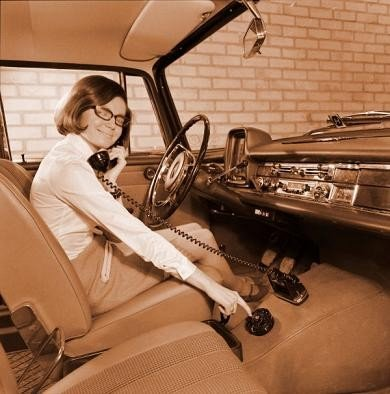
\includegraphics[width=10cm]{tanti-telefon}  
		\caption{\label{fig:tanti-telefon} Telefonul de mașină creat de Bell Labs
			\protect
			\cite{phone_lady}}
	\end{figure}
	

	La scurt timp după inovația adusă de către Bell Labs, AT\char`&T, compania americană specializată în telecomunicații, va avea să ofere servicii de telefonie mobilă și canale de comunicare pe zone restrânse. Dispozitivul oferit de către AT\char`&T era asemănător un transmițător radio. Era necesară apăsarea unui buton pentru a putea transmite un mesaj vocal, iar pentru a asculta interlocutorul, era necesară eliberarea butonului. Pentru a putea utiliza serviciile oferite de AT\char`&T în mașină, era nevoie de atașarea unui echipament care cântărea aproximativ 36 de kg.
	În 1949, serviciul telefonic susținut de AT\char`&T găzduia în jur de 5,000 de utilizatori, care realizau săptămânal aproximativ 30,000 de apeluri telefonice. Toate aceste apeluri telefonice erau gestionate manual de către operatori ai companiei AT\char`&T. 
	
	Un serviciu asemănător celui oferit de AT\char`&T, a fost creat în Regatul Unit și se numea Post Office Radiophone Service. Diferența facută de acest serviciu telefonic a fost modul în care erau gestionate apeluri telefonice. Deși erau gestionate în continuare de un operator, un apel telefonic putea fi realizat între oricare doi participanți din întregul Regat Unit. 
	
	Serviciul a fost creat în Manchester in 1959, adus în Londra in 1965, după care a fost distribuit în 1972 celorlalte orașe mari din Anglia.
	În anul 1983 va avea să apară primele telefoane mobile ce puteau fi ținute în mână. Primul producător de telefoane mobile a fost Motorola iar primul model a fost Motorola DynaTAC 8000x. Prețul său creștea până la 4000 de dolari, fiind un dispozitiv voluminos și greu (cântărind în jur de 4 kg)  având o baterie capabilă de a susține 30 de minute de convorbire. În ciuda dimenisiunii mari a acestuia, era considerat cea mai bună variantă din punctul de vedere al portabilității datorită faptului ca va avea să pună capăt dependenței cablurilor telefonice pentru a purta o convorbire.

	
	În anii 1990 au inceput să apară telefoane mobile aparținând generației a doua de dispozitive mobile. Acestea utilizau transmisie digitală, tehnologie ce aducea un plus de securitate și viteză peste transmisia analog. Odata cu această generație de dispozitive mobile, apar și SMS-urile (Short Message Service), prima utilizare fiind in 1993.
	În 1993, deși o teorie controversată, apare primul smartphone. IBM lansează modelul Simon. Acesta dispunea de: ceas, calendar, agendă telefonică, notițe, căsuță de email, auto-completare si touchscreen. (vezi Fig. \ref{fig:simon})
	
	
	
	\begin{figure}[H]
		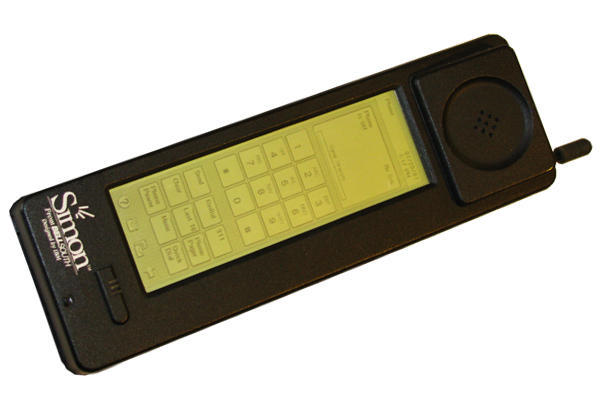
\includegraphics[width=8cm]{simon}  
		\caption{\label{fig:simon} Modelul de celular IBM Simon
			\protect
			\cite{ibm_simon}}
	\end{figure}
	
	
	După apariția modelului Simon, creat de IBM, dispozitivele mobile vor avea să urmeze un progres remarcabil în termen de funcționalitate, stil și cel mai important, forță de computație. 
	Telefoanele mobile au reușit să introducă în buzunarul oamenilor forța de procesare, de la utilizarea unui simplu serviciu de email sau calendar, până la utilizarea aplicațiilor ce dispun de inteligență artificiala. \cite{history_cellphones}
	\newline
	
	\section{Arhitecturi ARM}
	Pe parcursul timpului, calculatoarele și dispozitivele mobile au întâlnit mai multe arhitecturi ce au stat la baza componentei lor de baza, CPU. Acestea au fost dezvoltate ținând cont de necesitatea de computație de care are nevoie un sistem de calcul. Astăzi se pot enumera trei mari arhitecturi prezente în majoritatea dispozitivelor: arhitectura Intel x86, respectiv x86\char`_64 și arhitectura ARM. 
	
	Diferența între cele două mari tipuri de procesoare o face modul în care acestea gestionează computația. Procesoarele cu arhitectură Intel x86 și x86\char`_64 sunt bazate pe arhitecturi CISC (Complex instruction set computing) ce prezintă computație complexă, concentrată și plasată pe un număr relativ mic de nuclee. Acest lucru aduce avantajul forței mari de computație și multe operații per ciclu, însă crește proporțional consumul de energie. În contrast, procesoarele ARM sunt dezvoltate peste arhitectură RISC (Reduced Instruction Set Computing), care sunt reprezentate prin mai multe operații simple și scurte, rezultând în mai puține operații per ciclu dar și consum relativ redus de energie. 
	
	Neajunsurile arhitecturii de tip x86 sunt în continuare duse mai departe de calculatoarele cu sistem de operare Windows datorită compatibilității între versiuni, un factor important de care Microsoft ține cont. Acest lucru face pe moment imposibilă trecerea de la arhitecturi de tip x86 si x86\char`_64 spre arhitecturii ARM. 
	
	Deoarece dispozitivele mobile fiind relativ noi nu depind de arhitectura x86 și au putut fi dezvoltate peste arhitecturi ARM. Acest lucru este un factor important, datorită costului redus de energie pe care procesoarele ARM îl exercită. Datorită circuitelor mult mai scurte și a necesităților reduse la nivel de computație datorate numărului mic de tranzistori, acestea sunt de altfel reduse în dimensiune, aducând un plus in utilizarea lor ca și componenta a dispozitivelor mobile.
	
	Arhitecturile de tip ARM nu sunt noi. Acestea sunt prezente încă din anul 1980, aduse pe piață de compania Acorn RISC Machines Ltd. iar abrevierea provine de la Advanced RISC Machines. 
	
	Un avantaj important al arhitecturii ARM este posibilitatea de scalabilitate. Dat fiind raportul relativ îmbunătățit de performanță per watt, aplicațiile pot utiliza mai multe nuclee simple ale plăcii ARM și pot beneficia de consumul redus de energie. În timp ce procesoarele 
	Intel X86 realizează operatii complexe pe un număr redus de nuclee puternice computațional, procesoarele ARM pot împărți într-un număr mult mai mare de nuclee. Acest lucru devine optim în cazul unei aplicații software dezvoltată tinând cont de această modularizare si scalabilitate.
	\cite{arm_architecture_android}
	
	Lupta imbunătățirii capabilității procesoarelor și componentelor hardware ale telefonului mobile, sunt duse în scopul portării operațiilor de inferență a rețelelor neuronale complexe (Deep Neural Networks) de pe cloud chiar pe dispozitivul celular, în scopul diminuării timpului obținut pe parcursul etapei de transfer de date (TCP/IP și protocoale aferente). Avansarea componentelor de tip hardware aduc un plus doar de moment, urmând a-și pierde eficiența în timp. Pentru a obține o optimizare bună a serviciilor de inferență, trebuiesc luate în calcul diferite metode de accelerare a operațiilor. Începând de la arhitecturi scalabile și ne-consumatoare ARM, abstractizarea operațiilor responsabile de hardware și expunerea unei interfețe pentru utilizarea acestora eficient și până la optimizarea unor algoritmii în scopul sprijinirii arhitecturilor reduse in puterea de computație.
	
	Accelerarea inferenței rețelelor neuronale este un obiectiv luat în calcul în momentul actual de multe dintre companiilor producătoare de dispozitive mobile. Apple vine, începând cu modelul Iphone X, cu acceleratorul Neural Engine, specializat pe operațiile inferenței, iar Microsoft HoloLens vine cu HPU CNN. \cite{arm_ml}
	
	\section{Sistemul de operare Android}
	
	Android este un sistem de operare Open Source dezvoltat și întreținut de către compania Google. Google a cumparat în anul 2005 compania Android Inc., o companie ce se ocupa cu sisteme de operare pentru camere foto digitale și dispozitive mobile, cu scopul intrării pe piața dispozitivelor mobile. După 2 ani de la cumpărarea companiei, Google lansează sistemul de operare pe piață. 
	
	În momentul de față, 85\% din totalitatea utilizatorilor dispozitivelor mobile smartphone, utlizează sistemul de operare Android. 
	
	Ceea ce face sistemul de operare Android, un punct de interes în viziunea invățării automate, este arhitectura sa. Android are la bază o versiune a nucleului Linux, sistem de operare care face parte din familia UNIX. Sistemul de operare poate rula pe arhitecturi ARM. 
	
	Începând cu anul 2012, dispozitivele mobile Android sunt dezvoltate utilizând procesoare Intel iar mai târziu se vor stabili pe arhitecturi de 64-bit, ARM. 
	Forța pe care procesoarele dispozitivelor mobile o aduc, împreună cu sistemul de operare Android, ne permit utilizarea multor tehnici de învățare automată chiar pe sistemul telefonului. 
	
	Deși placa de bază a dispozitivelor mobile permite rularea unor computații complexe și utilizarea procesurilor și a firelor de execuție, acestea permit de altfel utilizarea plăcii grafice (GPU) în scopul realizării unor computații intense si distribuite.
	
	\subsection{Android System Developer Kit}
	
	Android System Developer Kit, sau Android SDK, este interfața expusă de Google, în scopul dezvoltării de aplicații și widgeturi pentru dispozitivele mobile Android, apărută în 2008. Android SDK este un tool ce face  funcționalitățile de bază ale telefonului mobil (cum ar fi camera, microfonul sau giroscopul) ușor de utilizat, oferă biblioteci programabile, condiții de compilare, depanare și emulare a modelelor de dispozitive Android. 
	Sistemul de operare poate fi împărțit în 5 componente:
	\begin{itemize}
		\item Aplications. Acestea sunt produsele finale la care au acces utilizatorii.
		
		
		\item Application Framework. Application Framework este baza programabilă care ușureaza utilizarea unor functionalități precum: camera video sau foto, activități, servicii de messaging, etc.
		
		\item Libraries. Penru a usura utilizarea bazelor de date, Secure Socket Layer, OpenGL, etc., au fost aduse la îndemâna programatorilor, biblioteci specializate în utilizarea acestor tehnologii.
		
		\item Android Runtime. Aplicațiile au nevoie de o masină virtuala pentru a rula. Android Runtime contine toate rutinele necesare pentru a compila și a rula o aplicație.
		
		\item Linux Kernel. Pentru a accesa componentele hardware ale telefonului, sistemul de operare folosește interefețe numite "drivers". Acestea sunt rutine ce opereaza low-level cu placa de bază.
	\end{itemize}
	
	\vfill
	
	Pe parcursul dezvoltăii proiectului Android, acesta a trecut prin diferite versiuni, fiecare aducând o extensie în materie de funcționalități și îmbunătățiri soft. Desi proiectul era orientat spre progres, dezvoltarea s-a făcut ținând cont de compatibilitatea anterioară. Astfel, versiunile noi ale sistemului de operare, pot rula aplicații cu o vechime mai mare decăt acestea.
	
	Prima versiune de Android a fost Astro 1.0. Aceasta rula pe modelul HTC Dream și deținea multe dintre aplicațiile care sunt înăa utilizate în ziua de astăzi. Printre aceste aplicații se numără Android Market, Gmail, Google Maps etc.
	La aprope doi ani după apariția versiunii Astro, apare versiunea 1.5 Cupcake. Aceasta rula pe un nucleu Linux 2.6, și a adus multe avantaje utilizatorilor și programatorilor. Această versiune a introdus widgeturi, animații și alte funcționalități la nivelul dispozitivelor cu Bluetooth.
	\newline
	
	Pe parcursul dezvltării, fiecare versiune apărută a adus o îmbunătățire in materie de funcționalitate sau interfață vizuală, insă un punct critic în dezvoltarea sistemului de operare și unul memorabil pentru învățarea automată, a fost versiunea 4.0, Ice Cream Sandwich. Această versiunea a fost lansată în anul 2011 și este bazată pe un nucleu Linux, versiunea 3.0. Pe lângă îmbunătățirile aduse interfăței vizuale și flexibilității de configurare, versiunea Ice Cream Sandwich introduce utilizarea algoritmilor inteligenți de detectare a feței și posibilitatea de a debloca telefonul utilizând recunoaștere facială. 	
	Acest punct marchează posibilitatea utilizării algoritmilor de învățare automată pe dispozitivele mobile, fiind un imbold spre avansarea învățării automate pe acest plan. Dezvoltarea proiectului a ținut cont din acest moment, de necesitatea utilizării algoritmilor inteligenti pe dispozitive mobile, astfel s-a pus accent pe accelerarea hardware si minimalizarea costului sistemelor inteligente. Avansarea componentelor hardware nu constituie întregul motiv pentru care utilizarea algoritmilor inteligenți a devenit posibila, ci și simplificarea si optimizarea acestora pentru a fi utilizați în parametri optimi de rulare.
	\newline
	
	Deși există alternative pentru dezvoltarea de aplicații pe dispozitive Android, interfața oferită de Google este cea mai populară ca și număr de utilizatori. Un aspect important al acestei interfețe, este flexibilitatea pe care o oferă, în materie de limbaje de programare. Aplicațiile Android pot fi dezvoltate pe baza Android SDK, utilizând limbajele de programare Java, C++ si Kotlin. \cite{android}	
	Android SDK expune modalități de a procesa imaginile preluate din camera video a dispozitivului. Aceste modalități, împreună cu bilblioteci specializate în computații distribuite utilizând forța GPU, ne permite utilizarea unor algoritm de invățare automată. 
	
	
	
\end{document}